\chapter{Introducción}
En el transcurso de los últimos años, es decir, desde la década de los años 2000 en adelante, ha habido un aumento considerable en el uso de energías renovables no convencionales para la obtención de electricidad en todo el planeta. El consenso internacional de avanzar en pos de un desarrollo sustentable para la humanidad y que esta, a la vez, sea amigable con el resto de las especies y los recursos naturales, marca la pauta sobre la manera correcta de hacer ingeniería. Considerando esto, la proyección está en que estas tecnologías continúen en un proceso de mejora continua y aseguren el bienestar de la sociedad.

De manera mas concreta las Energías Renovables No Convencionales (en adelante ERNC) corresponden a la energía solar, la energía hidráulica, la mareomotriz, undimotriz, geotérmica, biomasa y eólica. Para el alcance de este trabajo de tesis, el enfoque se centra en la energía eólica, que es aquella energía que se extrae del viento en movimiento.

El recurso viento posee la particularidad de ser extremadamente variable en todo su espectro de escalas temporales y espaciales, es decir, presenta fenómenos cíclicos distinguibles en cada una de estas escalas involucradas. Desde los cambios que tiene en la escala climática (ciclos planetarios, cambio climático) hasta la microescala (turbulencia, interacción con el terreno) y, por ende, la generación de energía a partir de este recurso es indistintamente variable. 
 

%Este hecho sustenta la necesidad de tener predicciones para la rapidez del viento lo mas cercanas a la realidad que se puedan, ya que variaciones en la potencia que puede generar un parque eólico puede significar la no rentabilidad económica de este, entre otros problemas como mantenciones correctivas o fallas en la planificación de la mantención preventiva de las turbinas y la aparición esfuerzos no deseados en el aspa.

Las zonas con mayor potencial eólico (i.e. aquellos lugares donde estadísticamente se tienen velocidades del viento lo suficientemente altas para que sea conveniente generar energía), son aquellas con terreno complejo, o sea, terreno con topografía no regular como las costas o montañas, debido a la aceleración que toma el viento al ajustarse a los contornos del suelo. Existe entonces una dicotomía o conflicto entre que los lugares mas aptos para poner parques eólicos, son al mismo tiempo los mas turbulentos y los más difíciles de predecir.

De este modo, surge la necesidad de buscar herramientas teóricas y prácticas para replicar el comportamiento y la rapidez del viento en su interacción con el terreno complejo y así también determinar la potencia eléctrica que se puede generar de esta.

Históricamente, se ha dependido de técnicas estadísticas (describiendo el viento a través de distribuciones de probabilidad) basadas en bases de datos que contienen registros del viento a lo largo de varios años. El problema con este método es que para terreno complejo, en donde el comportamiento del viento es en gran parte no lineal y heterogéneo, este no refleja el movimiento real ni los fenómenos complejos (como el desprendimiento de la capa límite o la mezcla turbulenta) dentro de la zona de interés. Aún asi, si se quisiera aplicar estos métodos estadísticos, el volumen de instrumentación necesaria sería inmenso para aplicarlo en zonas localizadas y por lo tanto, los costos asociados serían demasiado altos como para que se pudieran llevar a cabo en todos los lugares en donde se quisieran instalar turbinas.

Se busca entonces aplicar un método indirecto de bajo costo e impacto, lo que hace atractivo el predecir el comportamiento del viento a través de simulaciones numéricas, las cuales resuelven las ecuaciones que rigen el movimiento de la atmósfera. Estas ecuaciones son las llamadas ecuaciones primitivas y dan origen a una rama de la meteorología llamada predicción numérica del clima (Numerical Weather Predicción o NWP).

Las primera simulaciones atmosféricas datan desde el los años 20, en donde Lewis Fry Richardson logró hacer un pronóstico para 6 horas en dos puntos de Europa central. Este cálculo tardó cerca de dos semanas debido a que fueron realizados a mano. No fue hasta la década del 1950, con la llegada de los computadores, que este campo pudo desarrollarse mas intensivamente, principalmente gracias al trabajo desarrollado por el grupo de investigación de Carl-Gustav Rosby que logró un pronóstico operativo de 6 horas. Desde aquí en adelante, el avance exponencial de la computación y la sofisticación de las ecuaciones que modelan la atmósfera, han permitido tener pronósticos cada vez mas precisos y para períodos de tiempo cada vez mayores. 

En este estudio se simula la capa límite planetaria, que es la zona que está influenciada directamente por las condiciones del suelo y que en promedio tiene una altura de 1[km]. Los fenómenos que afectan a la capa límite, como por ejemplo la turbulencia originada por los obstáculos, la trasferencia de calor con la superficie terrestre o el intercambio de humedad con la vegetación, son características únicas de esta pequeña parte de la atmósfera. Por lo tanto la precisión que se tiene para estimar el comportamiento global del viento no es directamente útil para estimar el viento dentro de la capa límite, que es donde se concentra el interés para aplicaciones de energía eólica. 

Entonces, frente a esta latente necesidad de conocer el comportamiento del viento dentro de la capa límite sobre terreno complejo y aprovechando los avances en capacidad computacional que existen actualmente, es que se plantea el uso de simulaciones multiescala que permitan resolver desde las escalas planetarias hasta las escalas mas pequeñas relevantes para el caso de estudio y así obtener pronósticos fiables para zonas muy localizadas. Estos resultados no solamente serán útiles para la industria eólica, si no que también sientan las bases de una manera vanguardista para predecir dispersión de contaminantes, zonas de recirculación, evolución de incendios, control de heladas advectivas y radiativas, entre otros.

\begin{figure}[h]
	\centering
	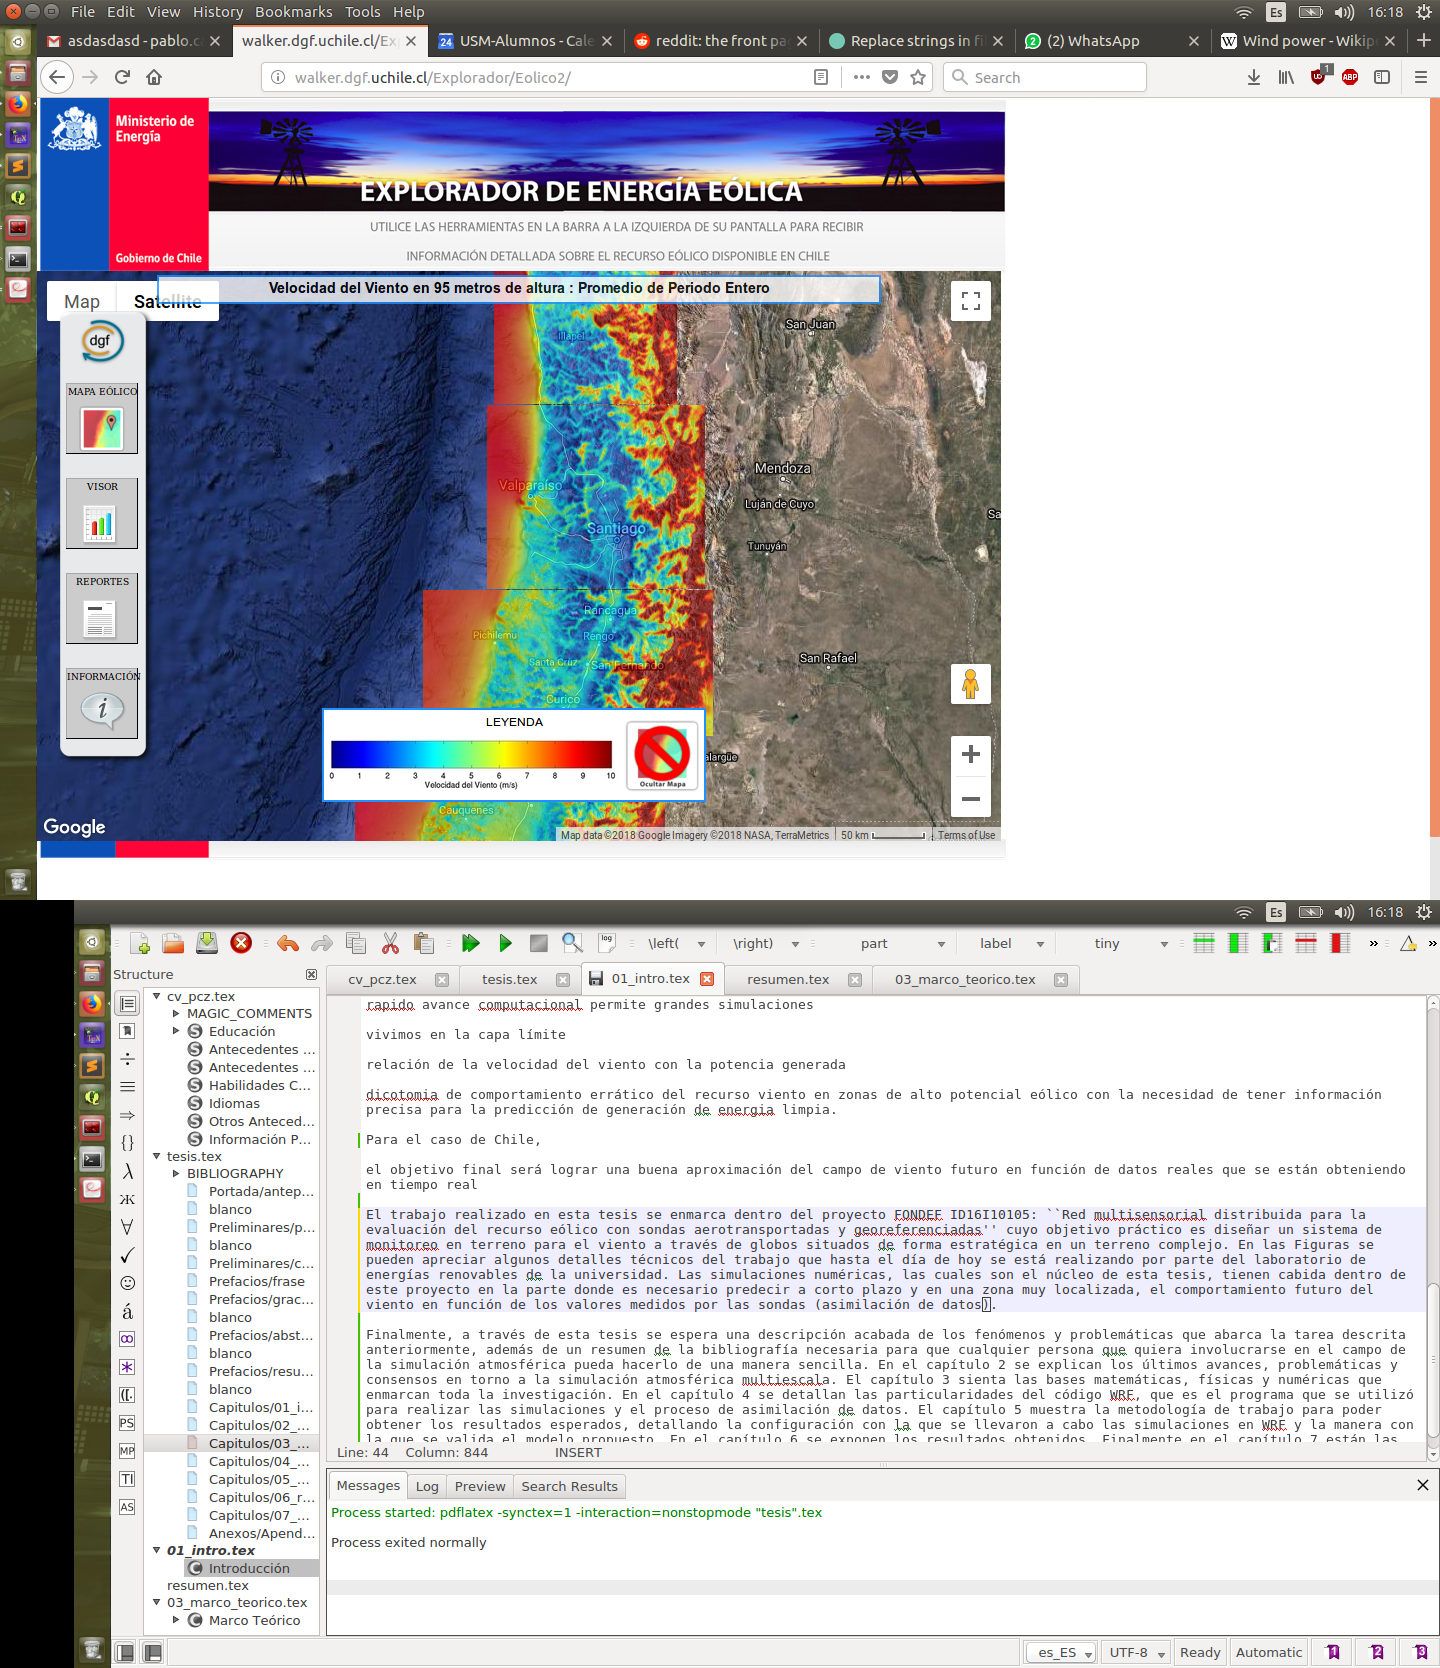
\includegraphics[width=0.9\linewidth,trim={1.4cm 28cm 15cm 3.4cm},clip]{Imagenes/01/explo}
	\caption{Interfaz online del explorador eólico de la Universidad de Chile.}
	\label{fig:01_explorador}
\end{figure}

Localmente en Chile cada año se están inaugurando nuevos parques eólicos debido al buen factor de planta que se poseen en ciertas zonas del país \citep{anuariocne2018}. Hasta la fecha ya se han instalado mas de 600 turbinas eólicas y la tendencia es a que este número siga aumentando. Actualmente Chile posee una potencia instalada de $23.315$ [MW], de los cuales un 7\% corresponde a energía eólica \citep{anuariocne2018}. El año 2017 se tenía un 6\% y el 2008 era menor a 1\%. De la mano de la instalación de nuevas plantas, está la simulación numérica realizada para tener una estimación de la cantidad de energía que se puede llegar a generar. En el 2010, la Universidad de Chile entregó a la comunidad la herramienta online llamada Explorador Eólico, en esta se muestra el potencial eólico que tiene gran parte de Chile, el cual fue simulado utilizando el modelo WRF. Algunos resultados de esta herramienta se pueden ver en la Figura \ref{fig:01_explorador}.

Si bien esta herramienta ha entregado a la comunidad información certera y que antes no existía, las simulaciones realizadas para el Explorador Eólico contemplaban mallas numéricas con una resolución horizontal máxima de 1 [km], lo que no es suficiente para resolver el comportamiento turbulento de microescala, ni para captar efectivamente las variaciones orográficas muy importantes para energía eólica. El comportamiento del viento a lo largo de una superficie de 1 [km$^2$] puede cambiar mucho, en especial si existe terreno complejo, y por lo tanto la ubicación o no de una turbina eólica requiere un análisis mas detallado del dominio.

El objetivo es entonces buscar una buena aproximación para el campo de viento en la capa límite en terrenos complejos y a alta resolución, a modo de tener una evaluación mas realista para la toma de decisiones en situaciones en donde el viento sea una variable crítica.

Debido a que en la capa límite es donde predominan los fenómenos de mezcla y turbulencia, es acá en donde los modelos presentan la mayoría de sus problemas operativos y desviaciones, y de hecho, el buen comportamiento del un modelo va a depender en gran manera de la habilidad del \emph{solver} para ajustar ciertos parámetros arbitrarios del código. 

Dado que la filosofía de este trabajo es utilizar la información original sin ser manipulada y evitar el ajuste de parámetros, es que se busca la manera de corregir los resultados numéricos a través de un proceso de asimilación de datos utilizando los valores paramétricos medidos en terreno.

La asimilación de datos es el proceso matemático mediante el cual se combina información de observaciones y de simulación numérica para obtener la mejor estimación del estado real de la atmósfera en un instante dado. Este proceso se utiliza cotidianamente en modelos globales o sinópticos para entregar la información sobre el clima que se presenta día a día en los noticieros.

Para los modelos meteorológicos mesoescala, el realizar asimilación de datos en la microescala no presenta beneficios, debido a que generalmente la resolución de estos modelos es gruesa en las cercanías de la superficie (la capa límite está pobremente resuelta), lo que se traduce en que la combinación entre observaciones superficiales y resultados numéricos no es fiable.

Sin embargo, y considerando esto como motivación para esta investigación, si se trabaja a resoluciones lo suficientemente altas como para tener información confiable en las cercanías de la superficie, si es posible realizar asimilación de datos en la microescala y por lo tanto mejorar los pronósticos del viento en la capa de superficie.

El trabajo realizado en esta tesis se enmarca dentro del proyecto FONDEF ID16I10105: ``Red multisensorial distribuida para la evaluación del recurso eólico con sondas aerotransportadas y georeferenciadas'' cuyo objetivo práctico es diseñar una red neuronal para monitoreo del viento a través de globos situados de forma estratégica en un terreno complejo. Dicha red de sondas cautivas constituye un sistema de acopio de datos multiparamétricos que alimentarán un modelo numérico como WRF. En las Figuras \ref{fig:01_detalle_fondef} y \ref{fig:01_sonda} se pueden apreciar algunos detalles técnicos del trabajo que hasta el día de hoy se está realizando por parte del Laboratorio de Energías Renovables de la UTFSM. Las simulaciones numéricas, las cuales son el núcleo de esta tesis, tienen cabida dentro de este proyecto en la parte donde es necesario predecir a corto plazo y en una zona muy localizada, el comportamiento futuro del viento en función de los valores medidos por las sondas (proceso de asimilación de datos).

\begin{figure}
	\begin{minipage}{0.5\linewidth}
		\centering
		(a)
	\end{minipage}
	\begin{minipage}{0.5\linewidth}
		\centering
		(b)
	\end{minipage}
	
	\begin{minipage}{0.5\linewidth}
		\centering
		\includegraphics[width=0.9\linewidth,page=3,trim={6cm 12.2cm 6cm 9.5cm},clip]{Imagenes/01/descrp}
	\end{minipage}
	\begin{minipage}{0.5\linewidth}
		\centering
		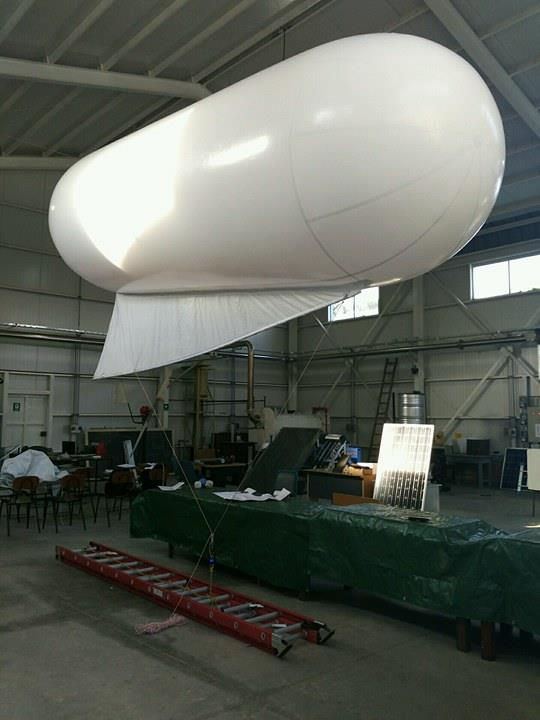
\includegraphics[width=0.7\linewidth,trim={0cm 0cm 0cm 0cm},clip]{Imagenes/01/prototipo}
	\end{minipage}
	\caption{Detalle del proyecto FONDEF ID16I10105. (a) Célula del sistema experimental de medición. (b) Prototipo en el laboratorio.}
	\label{fig:01_detalle_fondef}
\end{figure}

El objetivo final de esta investigación es implementar un sistema robusto que obtenga una buena aproximación del campo de viento futuro en función del ajuste pronóstico  datos medidos que se obtienen en tiempo real, mediante simulaciones numéricas multiescala realizadas con el software libre WRF y asimilación de datos 4D. La filosofía de simulación, será realizarlas de la manera menos manipulada posible, utilizando bases de datos públicas y evitando la asignación arbitraria de parámetros. Este enfoque ha sido poco investigado para la predicción y caracterización eólica en terreno real a alta resolución. 

\begin{figure}[h!]
	\centering
	\includegraphics[width=0.82\linewidth,page=5,trim={3cm 2cm 2.3cm 3cm},clip]{Imagenes/01/descrp}
	\caption{Esquema de la sonda FONDEF ID16I10105.}
	\label{fig:01_sonda}
\end{figure}

En el presente trabajo se brinda una descripción acabada de los fenómenos y problemáticas que abarca la tarea descrita anteriormente, además de un resumen de la bibliografía necesaria para que cualquier persona que quiera involucrarse en el campo de la simulación atmosférica con asimilación de datos pueda hacerlo de una manera sencilla. Como beneficio para la comunidad científica, los resultados obtenidos podrán ser utilizados como linea de base (o benchmark) para cualquier otra simulación futura a alta resolución, pudiendo dar pié a una nueva prueba canónica para modelos multiescala en operación continua.

%ACA VA LA CORRECCIÓN
\section{Hipótesis}

Mejorar la precisión de los pronósticos actuales para el viento a través de simulaciones atmosféricas multiescala de alta resolución en terreno complejo y la incorporación de un esquema de asimilación de datos 4D que vaya alimentando datos al sistema en tiempo real.

\section{Objetivos}
\subsubsection{Objetivo Principal}
\begin{itemize*}
	\item Lograr a través de la aplicación de asimilación de datos 4D multipunto en la capa límite atmosférica una mejora comparativa con respecto a los modelos existentes para la predicción de viento a alta resolución en terreno complejo en el modelo de código libre WRF.
\end{itemize*}
\subsubsection{Objetivos Secundarios}
\begin{itemize*}
	\item Acoplar dominios de microescala y mesoescala en simulaciones numéricas atmosféricas mediante una clausura de turbulencia tipo LES.
	\item Estudiar el uso e incorporar bases de datos reales de alta resolución para orografía y uso de suelo en el modelo WRF.
	\item Desarrollar y optimizar códigos relacionados con simulación atmosférica multiescala y asimilación de datos.
	\item Estudiar la influencia de la asimilación de datos en la capa límite considerando un solo punto y multipunto.
	\item Verificar y validar resultados obtenidos con aquellos presentes en el estado del arte y campañas de medición en terrenos reales.
	\item Generar una base de datos de resultados para terreno complejo real utilizable como benchmark para la comunidad científica. 
\end{itemize*}

\section{Estructura del Documento}
La estructura de esta tesis se organiza de la siguiente manera:
\begin{itemize*}
	\item Cap. 2: Se exponen los últimos avances, problemáticas y consensos en torno a la simulación atmosférica multiescala y asimilación de datos, que son el núcleo del trabajo realizado.
	\item Cap. 3: Sienta las bases conceptuales, matemáticas y físicas sobre las cuales se desarrolla la investigación. Acá se abordan: las leyes fundamentales de los fluidos, la dinámica atmosférica, la turbulencia, la capa límite planetaria, el método de simulación de grandes vórtices (LES) y la asimilación de datos.
	\item Cap. 4: Sienta las bases numéricas, es decir, se explica el funcionamiento del software  libre WRF.
	\item Cap. 5: Muestra la filosofía y configuración de los 4 experimentos realizados: 2 casos para terreno plano (donde uno sirve como validación y el otro analiza la asimilación de datos) y dos casos para terreno complejo (sin y con asimilación). Además, se detalla la metodología para la obtención y presentación de resultados.
	\item Cap. 6: Se presentan los resultados mas relevantes.
	\item Cap. 7: Conclusiones, trabajo futuro y aspectos que quedan abiertos a la mejora.
\end{itemize*}
